

\chapter{Molecular Aggregates}

\section{Experiment}

\textit{spektral, fl. Lifetime, ensemble, TDBC ?
}

\textit{Bestimmen sie die Konzentration, ab der sich Aggregate bilden. Über wieviel Chromophore ist der Zustand delokalisiert?}

%\section{Experiment}

\section{Quantenmechanik gekoppelter Systeme\protect\footnote{Parson, Kap. 7.1 und 8.1, Stephan Wiesneth}} 



Two molecules should be so close to each other that after excitation, it is no longer possible to determine which of the two molecules is excited. The excitation is thus delocalized via the system, which is also called \textit{exciton}. The exciton interaction does not physically differ from the interaction at resonance energy transfer.

The state wave functions are again represented as a combination of the wave functions of the individual molecules:
\[ \Psi_A = \phi_{1a}\chi_{1a}\phi_{2a}\chi_{2a} \]
\[ \Psi_B = C_1\psi_1 + C_2\psi_2 = C_1\phi_{1b}\chi_{1b}\phi_{2a}\chi_{2a} + C_2\phi_{1a}\chi_{1a}\phi_{2b} \] 
$\Psi_A$ corresponds to the basic state, $\Psi_B$ to the excited state of the dimmer. The $\psi_1$ and $\psi_2$ are not stationary states here, since the energy is quickly transferred back and forth between the molecules.

The energy of the ground state is calculated as follows:
\begin{equation}
    E_A = \langle\phi_{1a}\phi_{2a}\lvert\tilde{H}_1+\tilde{H}_2+\tilde{H}'\rvert\phi_{1a}\phi_{2a}\rangle = E_{1a}+E_{2a}+\langle\phi_{1a}\phi_{2a}\lvert\tilde{H}'\rvert\phi_{1a}\phi_{2a}\rangle.
\end{equation}
The last term is very small compared to the first two if the molecules are uncharged and have a small transition dipole moment.

For the energy of the excited state results
\begin{equation}
    E_B = \lvert C_1\rvert^2 E_1 + \lvert C_2\rvert^2 E_2 + \langle C_1\psi_1 + C_2\psi_2\lvert\tilde{H}'\rvert C_1\psi_1 + C_2\psi_2\rangle
\end{equation}
For a more precise calculation of the last term the stationary Schrödinger equation $\tilde{H}\Psi_B = E_B\Psi_B$ is used. This is multiplied once by $\psi_1*$ and once by $\psi_2*$. This gives the following system of equations:
\[ C_1 \left [\langle\psi_1\lvert\tilde{H}_1\rvert\psi_1\rangle+\langle\psi_1\lvert\tilde{H}'\rvert\psi_1\rangle - E_B\right] + C_2\langle\psi_1\lvert\tilde{H}'\rvert\psi_2\rangle = 0 \]
\[ C_1\langle\psi_2\lvert\tilde{H}'\rvert\psi_1\rangle + C_2 \left [\langle\psi_2\lvert\tilde{H}_2\rvert\psi_2\rangle+\langle\psi_2\lvert\tilde{H}'\rvert\psi_2\rangle - E_A\right] = 0 \]
The non-trivial solution is obtained by equating the zero:
\[ \begin{vmatrix}
    H_{11} - E_A & H_{21} \\
    H_{21} & H_{22} - E_B
   \end{vmatrix} = 0 \] 
Where $H_{11}=E_1+\langle\psi_1\lvert\tilde{H}'\rvert\psi_1\rangle$, corresponding for $H_{22}$ and $H_{21}=\langle\psi_2\lvert\tilde{H}'\rvert\psi_1\langle$. This gives you two possible values for $E_{B\pm}$, as well as two wave functions $\Psi_{B\pm}$:

\begin{equation}
    E_{B\pm} = E_0 \pm \frac{1}{2}\sqrt{\delta^2 + 4H_{12}^2}  
\end{equation}
\begin{equation}
    \Psi_{B\pm} = \sqrt{\frac{1+s}{2}}\cdot\psi_1 \pm \sqrt{\frac{1-s}{2}}\cdot\psi_2
\end{equation}
The newly introduced variables are $\delta = H_{11}-H_{22}$, $E_0 = \frac{H_{11}+H_{22}}{2}$ and $s = \delta/\sqrt{\delta^2+4H_{21}^2}$. In a dimer the excited states of the individual molecules are thus split into two new energy levels.
\begin{figure}
    \centering
    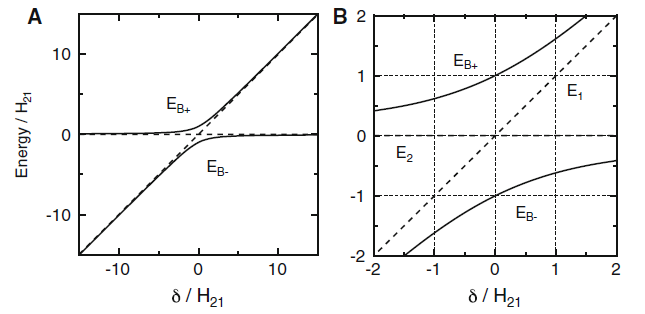
\includegraphics{\currfiledir/avoided_crossing.png}
    \caption{Energies of the two new states depending on the energy difference of the single excited molecules}
    \label{avoided_crossing}
\end{figure}
In figure \ref{avoided_crossing} it can be clearly seen that the energies of the states are never identical, which is also called \textit{avoided-crossing}.

\section{Spectroscopy of dimers\protect\footnote{Parson, ch. 8.2}} 

Which spectroscopic signature do coupled
Fluorophores?

\section{Antenna complexes\protect\footnote{Parson, section 8.5}} 

In nature, coupled fluorophores are found in
chlorophyll-antenna complexes. Why?




\printbibliography[segment=\therefsegment,heading=subbibliography]
